\documentclass[letterpaper,10pt,titlepage, onecolumn, compsoc]{IEEEtran}
\usepackage{graphicx}                                        
\usepackage{amssymb}                                         
\usepackage{amsmath}                                         
\usepackage{amsthm} 
\usepackage{soul}

\usepackage{alltt}                                           
\usepackage{float}
\usepackage{color}
\usepackage{url}

\usepackage{balance}
\usepackage[TABBOTCAP, tight]{subfigure}
\usepackage{enumitem}
\usepackage{pstricks, pst-node}

\usepackage{geometry}
\geometry{textheight=8.5in, textwidth=6in}

%random comment

%signature page formatting

\newcommand{\cred}[1]{{\color{red}#1}}
\newcommand{\cblue}[1]{{\color{blue}#1}}

\usepackage{hyperref}
\usepackage{geometry}

\title{Team LibNav \\ Design Document \\ CS Senior Capstone \\ \vspace{2mm}\small CS461 (Fall 2016)}
\author{Authored by \\ Nathan Healea, Stephen Krueger, Matthew Zakrevsky}
\date{November 14, 2016}
\begin{document}
% Title page
\maketitle

% Abstract
\section*{abstract}
Currently, the Oregon State University Valley Library's flat, un-interactive map fails to provide visitors the information needed to navigate the library effectively. Visitors struggle to navigate to marked locations and find places with desired attributes. In this design document, functionality, user interfaces, and database schema are design with specif view points in mind and provide detail specification for development.
\newpage

% Table of Contents
\tableofcontents
\newpage

% Overview
\section{Overview}

% Overview: Scope
\subsection{Scope}
LibNav is an interactive map web application to help provide navigation guidance to visitors of The Valley Library at Oregon State University. Student, Faculty, staff, and community members struggle with navigating the Valley Library to find location to study or to locate resources.  Visitors of the library also seek out specific attributes or resources when reserving study room online or when looking of a place to study independently. LibNav is designed in a way to help locate desired resources and to make a visit to the library a success.

% Overview: Purpose
\subsection{Purpose}
With resource continuously being added or removed locating them can be a problem. The Valley Library uses un-interactive maps that quickly become out-of-date when these resource change or when renovation to the building take place. LibNav purpose it solve these problems by providing two main functionalities in the web application. A administration dashboard, named Librarian Administration Dashboard (LAD), allows staff member to add location into the system with relative attributes and tags. This allows user to search for a location with desired attributes they are looking for. When a librarian staff member creates a location they will be able to draw that location on the map and have it data points be saved to later be used to indicate to a visitor were that location is located.  The second part is the Interactive Map. This allows visitor to found out information about a location, gives them the ability to search for desired attributes in a location, and to get directions to their desired location from their current position.  

% Overview: Intended Audience
\subsection{Intended Audience}
This document is intended for technical developers and stakeholder who have prepared and will use the document to develop the LibNav web application. This document provides detail information and diagrams towards functionalities, and designs that clearly layout the functions and User interface to be develop by technical developers. This document also provides detailed overview of each component that will be developed for stakeholders to understand more technical information and to help monitor the progress of the web application development.  

% Definitions: to be filled in by all members
\section{Definitions}
Oregon State Web Accessibility Guidelines: The design guidelines for websites hosted in the Oregon State University domain that describe web page layout that conforms with the Americans With Disabilities Act.

Document Object Model(DOM): Programming interface that defines modifying HTML and XML documents

Central Access Service(CAS):The login portal used to restrict access to protected Oregon State University websites.  

Scalable Vector Graphic(SVG): This is an image format that has built in XML data that can be modified and edited.

Attribute Tags: Keywords and phrases that will be used to describe different locations in the library. These will be stored in the database for use by the search functions

Regular Expressions: a sequence of characters that define a search pattern. 

ONID: Oregon State University Online Identifier and mail services.


% User Interface (UI)
\section{User Interface}

% UI: Librarian Administration Dashboard (LAD) (Nathan)
\subsection{Librarian Administration Dashboard (Nathan)}
Librarian Administration Dashboard (LAD) is the main data entry point for the LibNav Interactive map. The design of the user interface focuses on administrator, library staff, and student staff how will be managing and inputting majority of the information into the system. Since there is a wide variety of how technical a user might be, clean, easy to understand control will be implemented. To handle the structure functionality of LAB, built in css classes from Foundation will handle keeping the the display clean and functional. Foundation will provide css function for UI controls and styling, and endure the DOM elements will not overlap onto their DOM elements.

In figure 1 navigation around the LAD is laid out in clear way with navigation located at the top and left side of the web browser. 

The top navigation bar will provide link to main pages within the application, for example, the homepage, login\/logout links, and to the Interactive map. The top navigation will be it own file that will allow for easy edits to the information that needs to be displayed in the top navigation. This file name will be lab\_navagation. To build the top navigation Foundation CSS classes like top-bar, top-bar-left top-bar-right, and menu vertical will be used. 

The left sidebar will direct a user to the correct forms for inputting information. This sidebar is also designed in a way that additional links to forms or data editing can be added throughout the life cycle of the project and will reside in its own on file name lab\_sidbar. To keep the sidebar in place and display properly Foundation CSS classes like side-nav will be nested in div with a column class.

The main area of the LAB will allow relative information to be displayed for the user, for example  Role Management Form, Location Form, and lists of Known and Unknown location that can be selected for editing or deletion. This will be files that will contain the lab\_sidebar and the lab\_navagation. This file name will correspond to the information that will displayed in the main area, for example Location Form will contain the HTML structure and link in and call js functions for data sanitation and will be named lab\_location\_form.

\begin{figure}[h!]
\centering
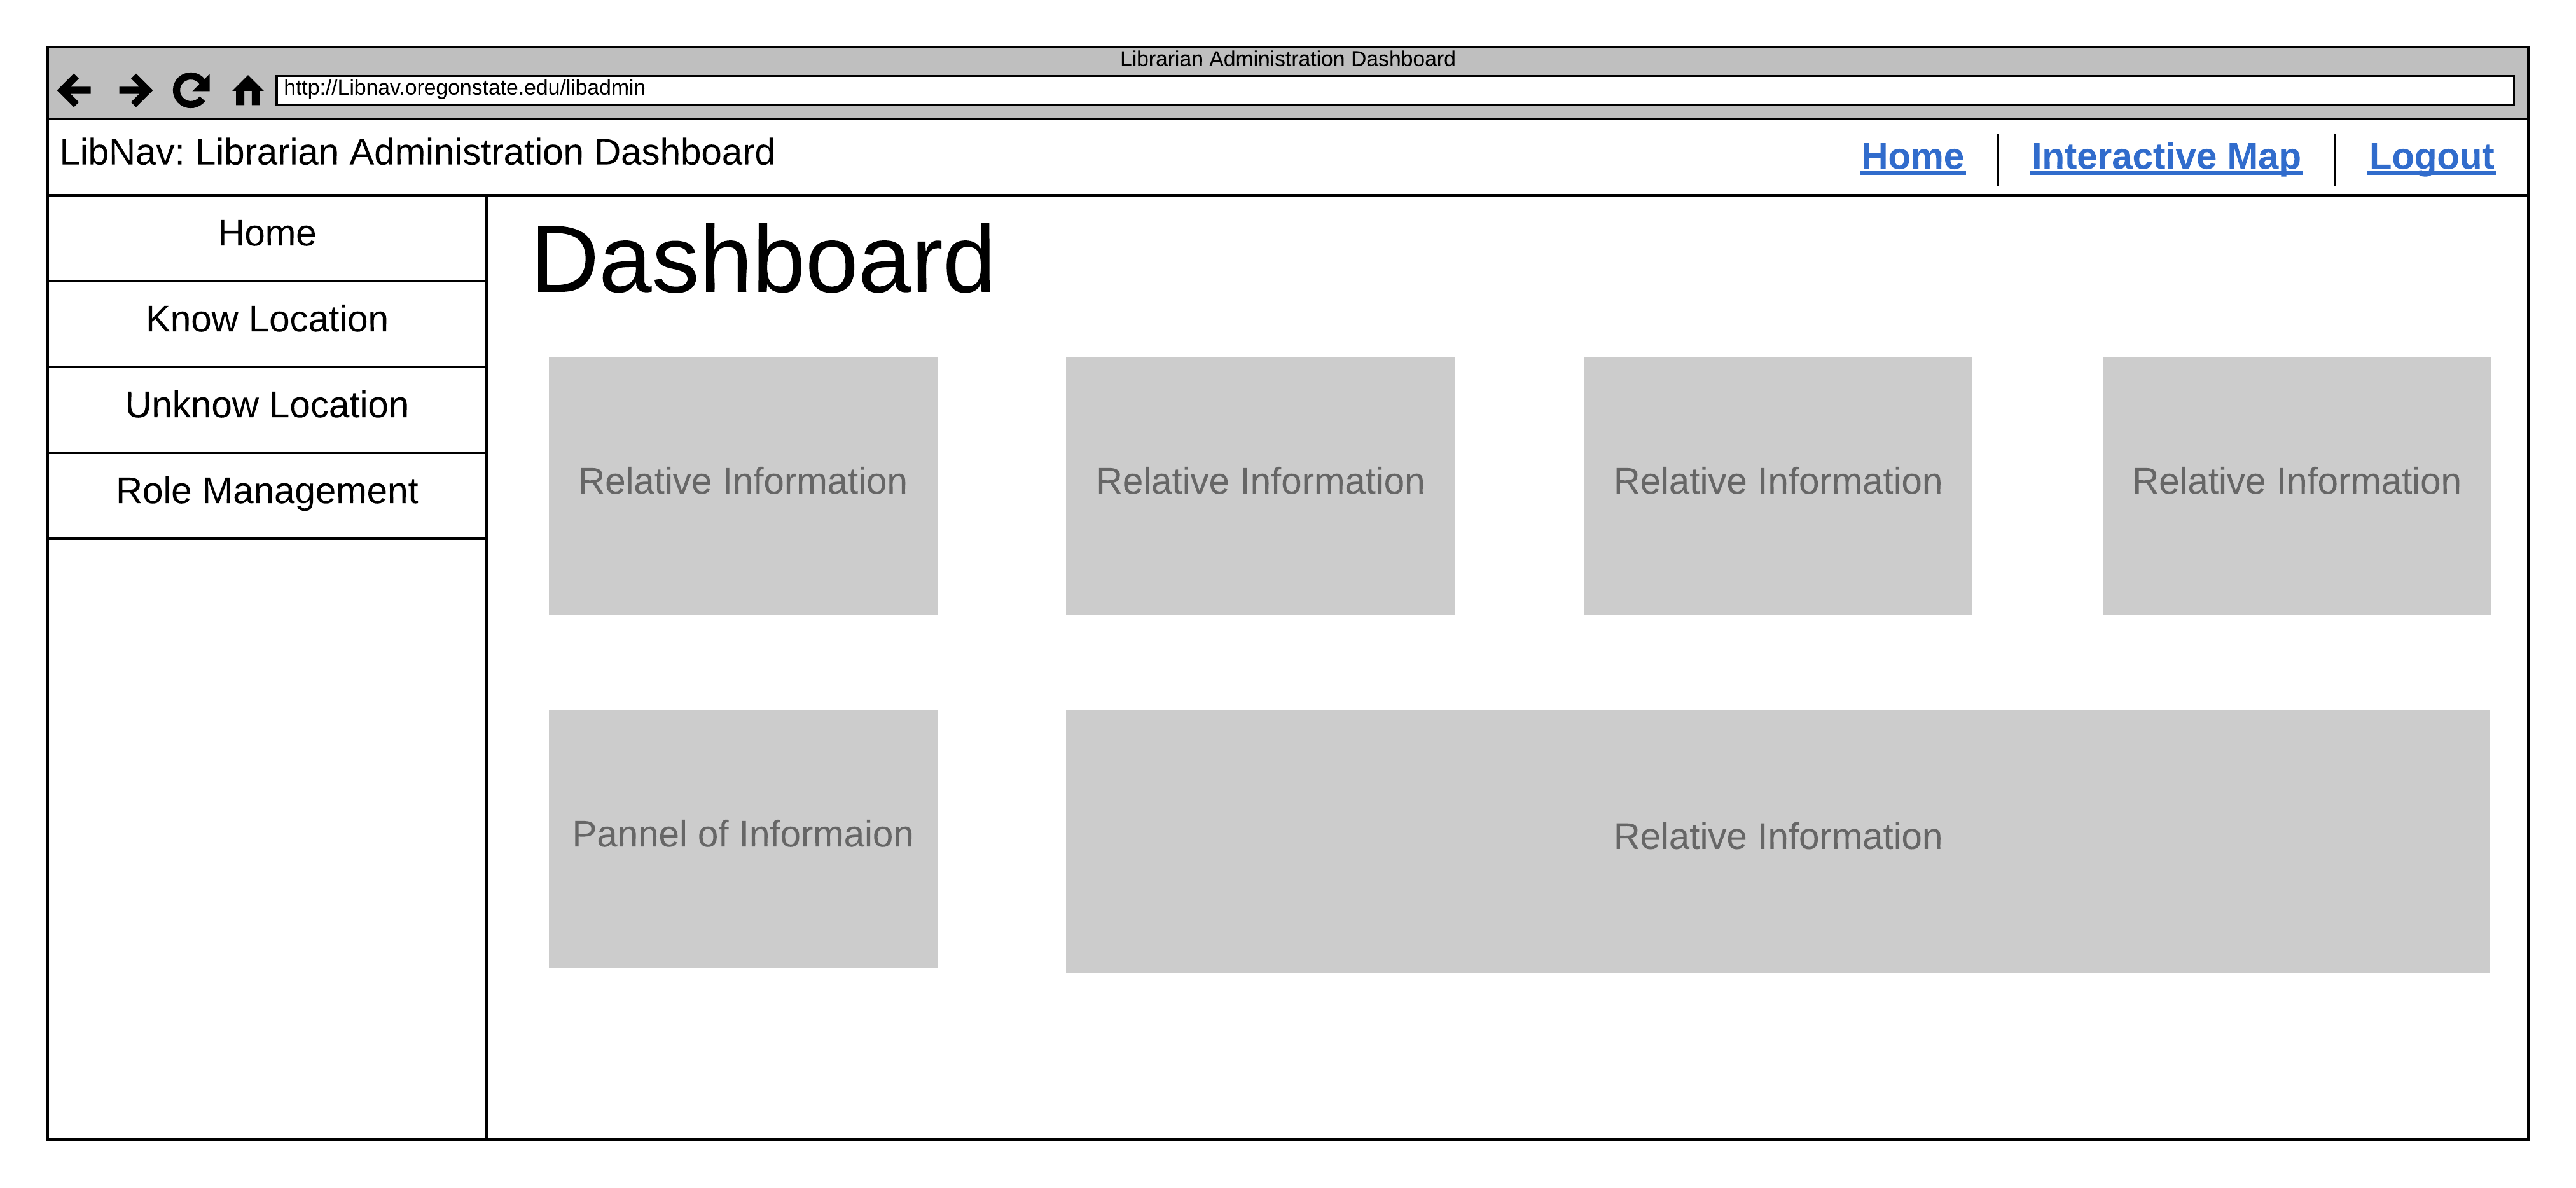
\includegraphics[scale=.45]{images/librarian-administration-dashboard.png}
\caption{Librarian Administration Dashboard User Interface}
\label{fig:method}
\end{figure}

% LAD: Map Drawing and Editing (Matthew)
\subsubsection{Map Drawing and Editing (Matthew)}
\subsubsection{Drawing}
For drawing new structures on the map, a new location will have to be created in order to save data to the database. This form structure will include a name and all necessary attributes to needed in order to create a space. The the bottom of this form will be a button to add new location. Once clicked, the view changes and the users will be presented with the map and a small window with a save button and a list of commands that can be used to draw lines and shapes on the map. After the user is done drawing the map location a button to save changes will need to be pressed in order to return to the form and submit the final changes. The final query will be then be sent to the database and inserted into the correct tables.

\subsubsection{Editing (Matthew)} 
In this Dash board the user will be presented maps that have been uploaded for use by the library staff. By selecting the edit button the user will be presented with a list of maps that can be modified. These maps will be loaded with all locations that have been previously created and populated in the database. Within this screen, a navigation dash board with a drop down menu of all locations on this map. By selecting a location, an HTML form of all preexisting data will be populated and will be shown in the form so that the information will be edited. Depending on the user’s role, certain pieces of the form can be edited such as the keyword tags and space descriptions, whereas full user access will allow full editing of the form. 

In addition when a user has full access to the Administrator Dashboard the form will also contain an edit button. When pressed, the view changes and the users will be presented with the map,  the location to be edited, and a small window with a save button and a list of commands that can be used to draw lines and shapes on the map. When clicked , the save button will return to the standard editor dashboard with the prepopulated form to allow the user to submit their changes. 

On the system side this form will query the database for all information that corresponds to the selected location that is being edited. With the query the the Javascript will parse the data and will populate the various text boxes within the form and any shapes on the map. When editing the map onclick javascript functions will be used to perform the required actions and when the map edits are saved the onclick functionality will be removed and the form can be submitted which will result in an insert data query to populate the data in the database, including all edited shape data.

All drawing will be done within the D3.js built in commands with d3.select.append functions. These drawing can be saved directly into the svg or saved as JSON objects to be saved in the database.

% LAD: Location Form (Nathan)
\subsubsection{Location Form (Nathan)}
Location Form are the main forms that user will use input information into the system to create Know and Unknown location. This form has been designed in a way where a non-technical user can input the data to create a new location. This for will consist of a HTML structured from at the top with a map of the library on the bottom with controls to draw location on the map. 

Location forms have been separated into four different types of locations: Know, Unknown, Rooms, and Service Point to help guild users to input the correct information.

\textbf{Know Location Form:} is information regarding fixed structures in the Library such as bathrooms, and emergency exits. This form will be comprised of the following input fields: Location name, Floor, Attribute, Tag, and Mark Location.

\textbf{Unknown Location Form:} is information regarding non-fix location in the Library such as Learning Commons, South wall tables, etc. This form will be comprised of the following input fields: Location name, Floor, Attribute, Tag, and Marked Location

\textbf{Room Location Form}: is information regarding fixed rooms in the Library such as study rooms, classrooms, offices, etc. This form will be comprised of the following input fields: Room Name, Floor, Room Number Room Capacity, Attribute, Tag, and Marked Location.

\textbf{Service Point Location Form:} is information regarding structure tied to services in the Library such as Circulation Desk, Special Collection \& Archives Research Center (SCARC), etc. This form will be comprised of the following input fields: Service Point Name, Floor, Room \#, Server URL, Attribute, Tag, and Marked Location

Below are details regarding the input fields, construction and validation.

\textbf{Location/ Service Point/ Room Name:} is a text box created using HTML label and input tags. This file will only accept alphanumeric entries that will be validated using Approved.js format function with a regular expression.

Type has been removed from the project and is now incorporated in different types on forms.
\st{Type: is a drop down menu what will consist of location types, example: Unknown, Known, room, service. This will be built using HTML label, select, and option tags. Validation for this input field will use Approved.js isEmpty() to ensure that one of the options have been selected. The options to select from will come from the room type database table. }


\textbf{URL:} will take a related url to that location. This could be a URL for a specific server, or to a registration form for a study room and will be created using HTML label and input tags. Data for this field will be validated by URL functionality from Approved.js.

\textbf{Room Number:} is an input format that will take the number of the room, office, or known location. It will be created using HTML label and input tags and be validated for alphanumeric formatting by Approved.js

\textbf{Attributes:} is a text box that will take a list of attributes for a given location. This will be a created by HTML label and input tag. Validate.js will use regular expression that the information will only contain letters. Since multiple values will be entered into the textbox custom parsing functionality will be writing to split text up on ‘,’.

\textbf{Tags:} will operate like Attributes using HTML input and labels with regular expression to check for only letters. It will use the same parsing functionality as Attributes to split the text on ‘,’.

\textbf{Save Button:} will make a request back to the control once all the form information has been validate and filled out. This information will be based back to the controller in a json object using POST.

textbf{Clear Button:} will clear all information that has been inputted into the from including the locations drawn on the map.

\text{Cancel Button:} will clear the from and redirect the user back to the LAB main page.

\begin{figure}[h!]
\centering
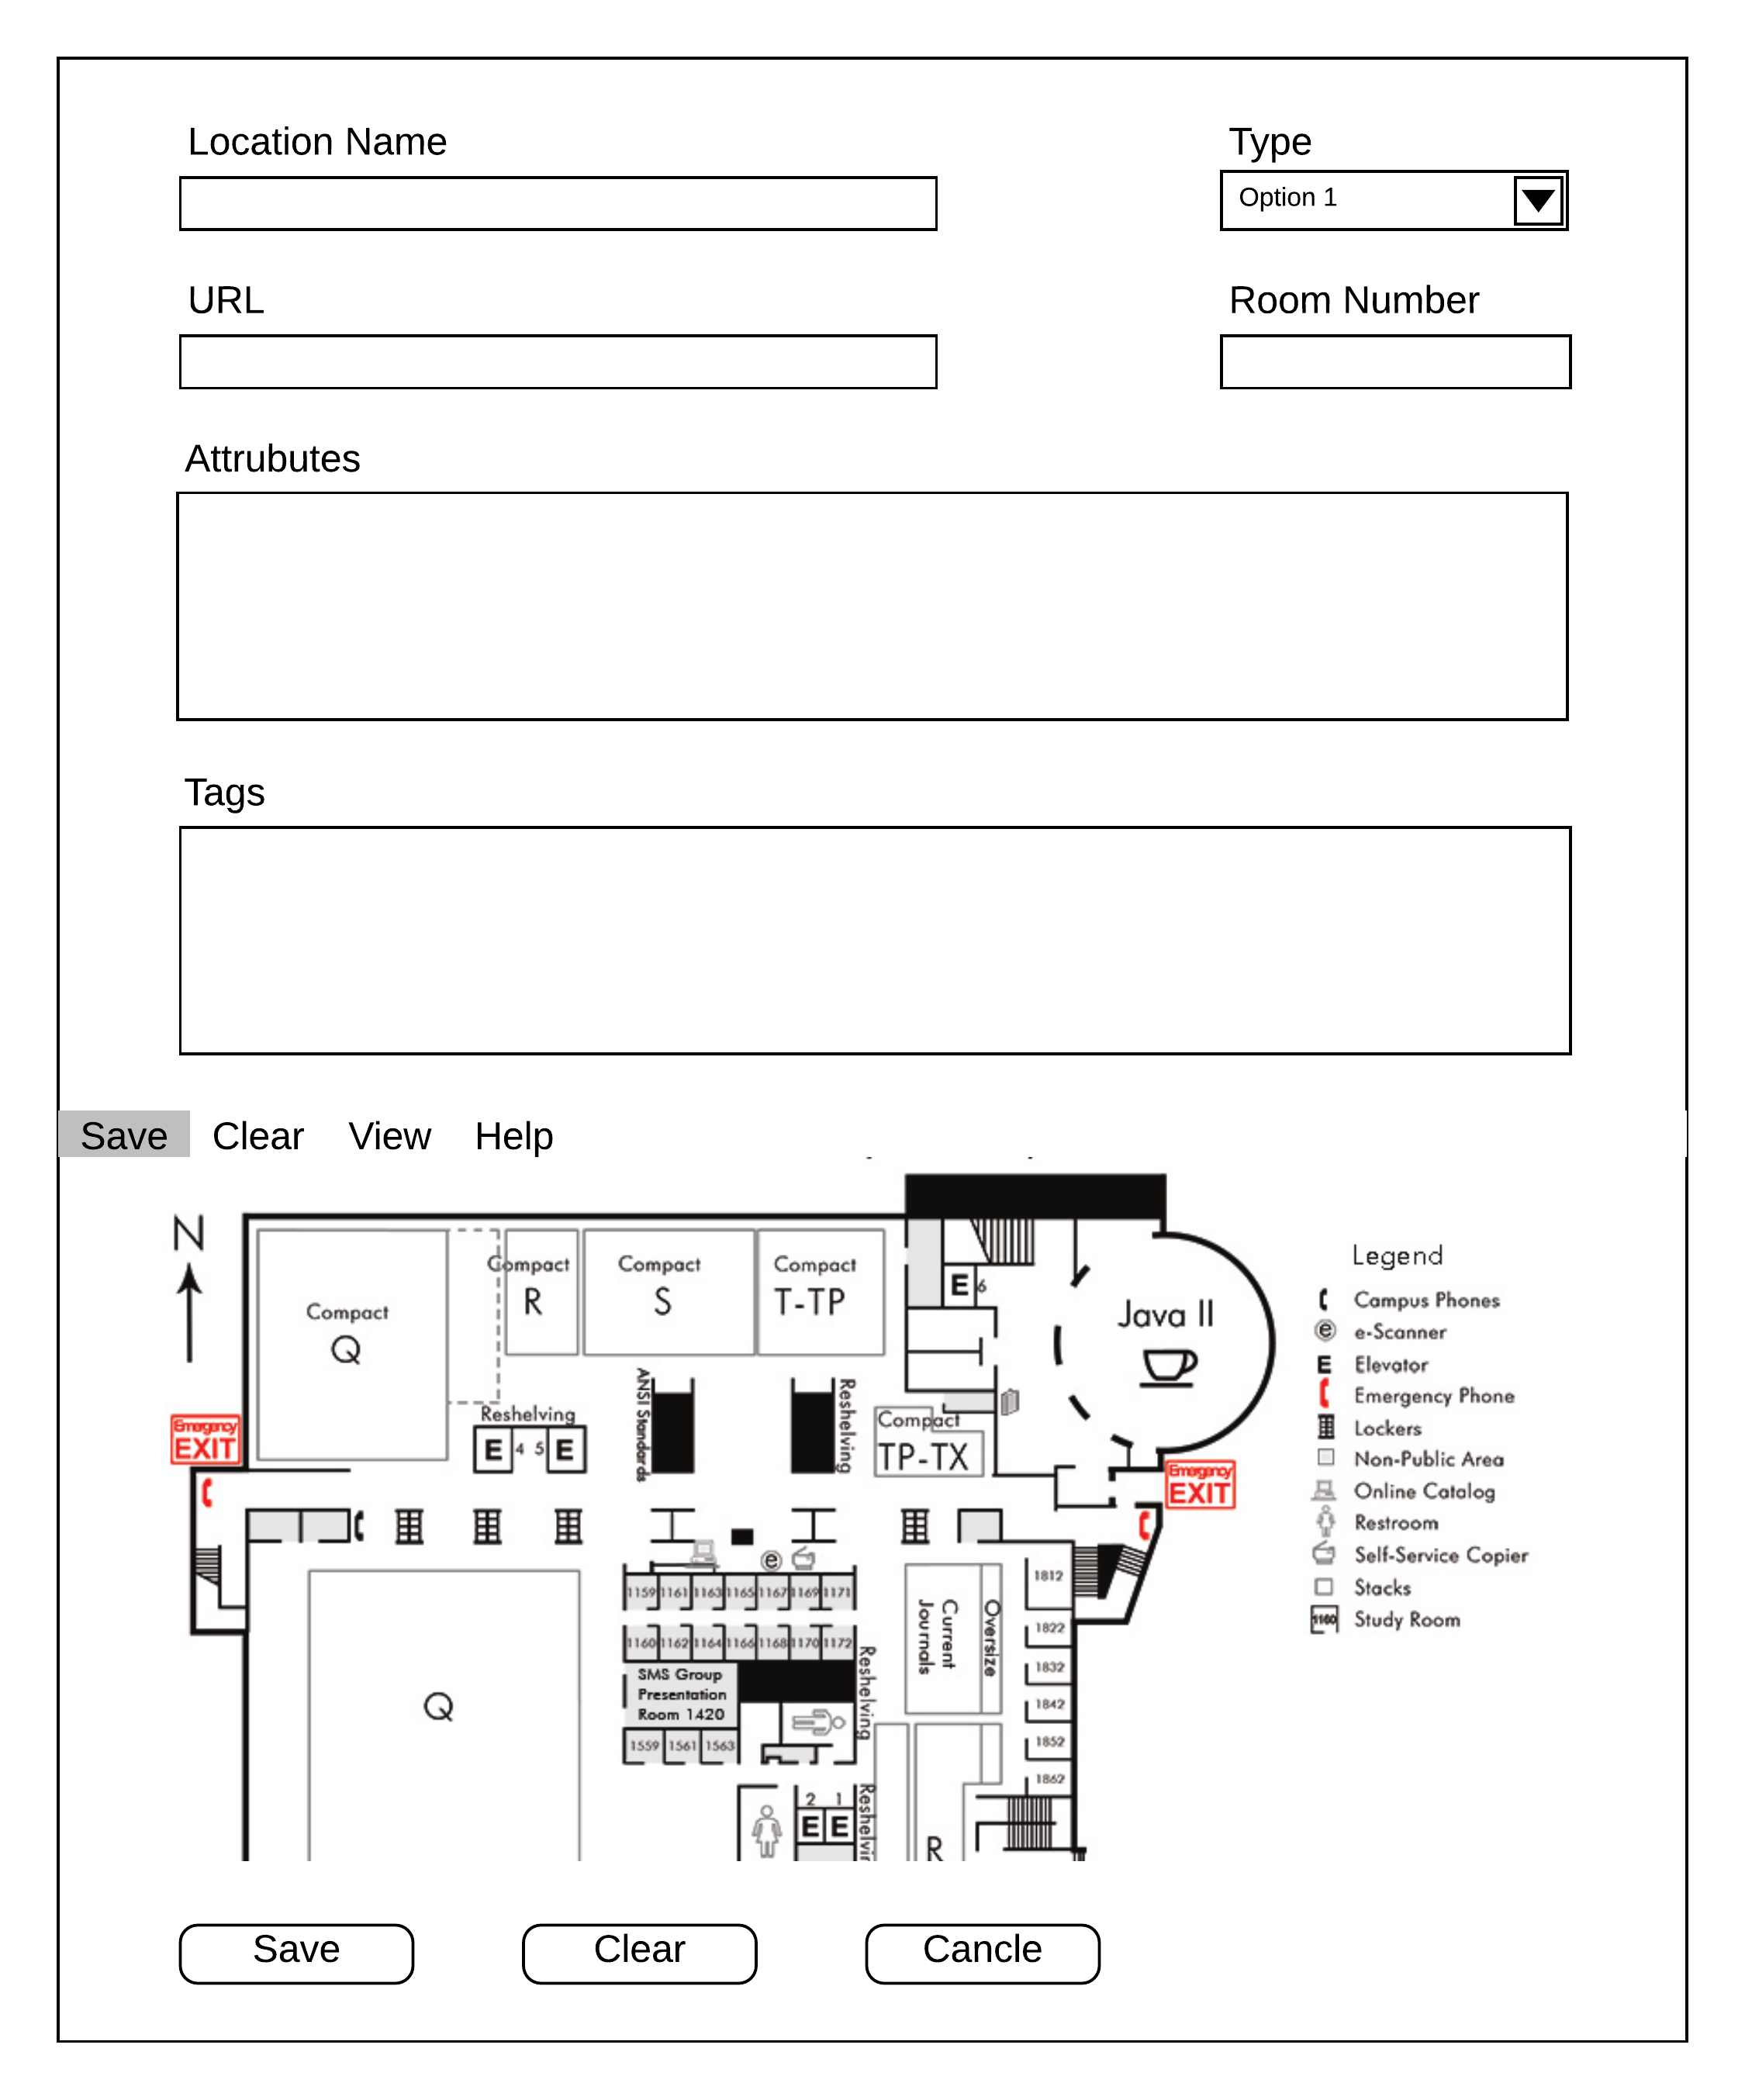
\includegraphics[scale=.45]{images/location-form.png}
\caption{Location From User Interface}
\label{fig:method}
\end{figure}

% LAD: Role Assignment Form (Nathan)
\subsubsection{Role Assignment Form (Nathan)}
The Role Assignment Form will allow an authorized administrator to grant access to a user. The design in a way that a non-technical user will be able to grant access to the site when needed. This form will consist of three two in input field. 

User name: will accept the end of the extended user in which the role will be assigned to.  It will be consists of an HTML label and input tag. This is be validated using validate.js regulator expressions to check that only letter have been entered.

Role: will be a dropdown menu constructed from HTML label, select, and option tags. Validate.js will check that an option has been selected by using isEmpty function.  

Save Button: will save the information inputted into the from after the form has been validated. The information will be passed to the controller in a json object using the POST method. This will consist of a HTML button tag colored green. 

Clear Button: will clear all information that has been selected and inputted into the form . This will be created using the HTML button tag colored yellow for indication. 

Cancel Button: will redirect the user back to the LAB homepage. this button will be constructed using the HTML button tag and colored red.

\begin{figure}[h!]
\centering
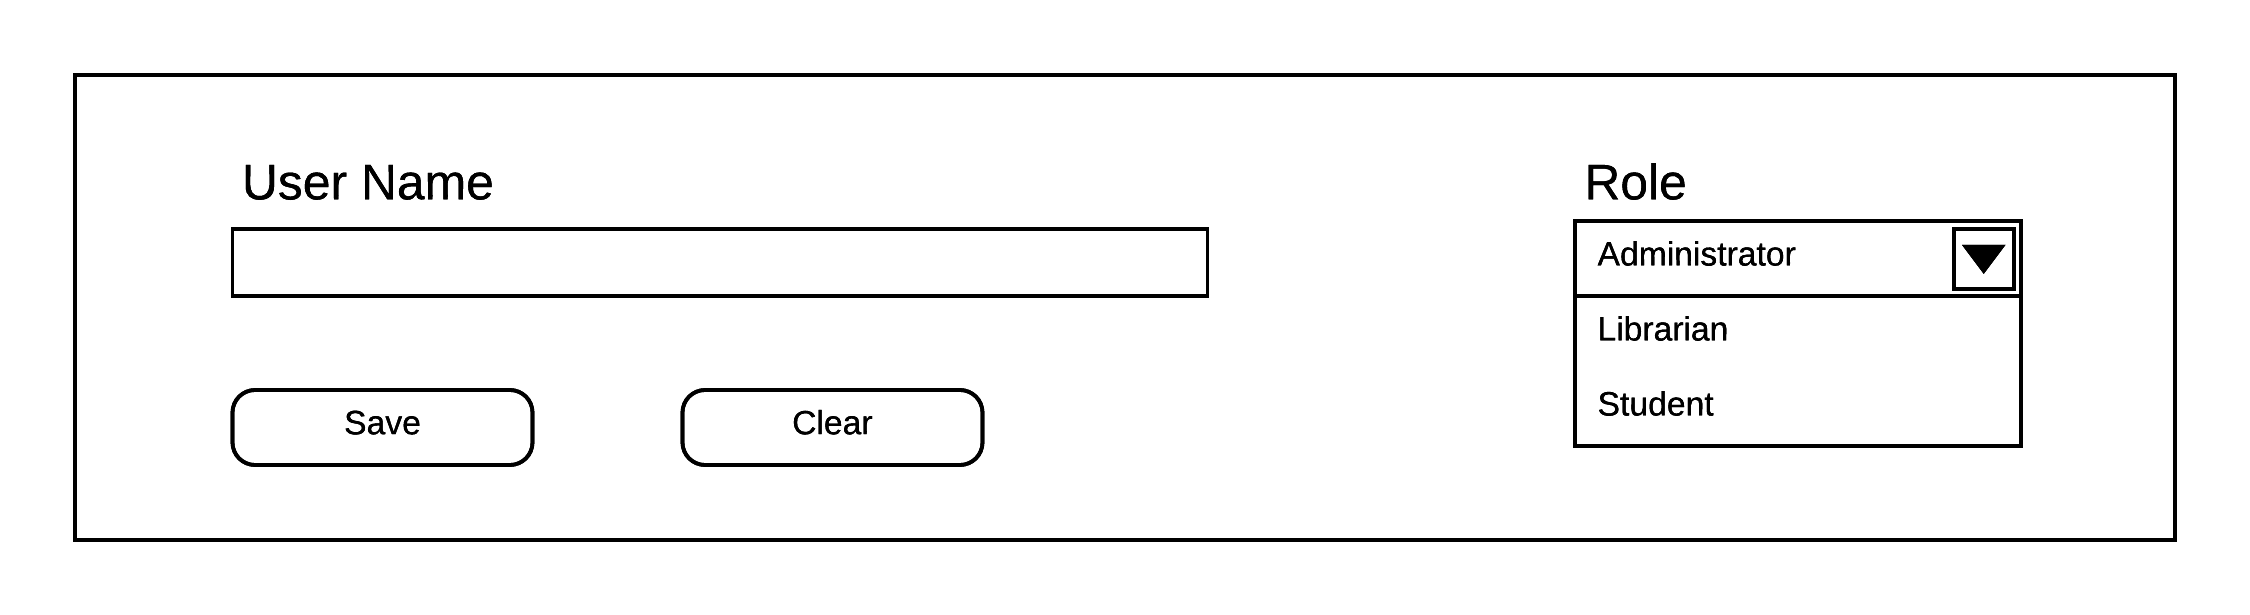
\includegraphics[scale=.6]{images/role-assignment-form.png}
\caption{Role Assignment Form User Interface}
\label{fig:method}
\end{figure}

% UI:  Interactive MAP (IM) (Nathan)
\subsection{Interactive Map (Nathan)}
The Interactive Map is the main part of the LibNav application. The design of the user interface for the interactive map focus on visitors of The Valley Library how will be selecting location they wish to navigate to. In order to make the Interactive map user friendly for both technical and technical the user interface will consists on a minimalistic design to help keeping buttons easy to click on, information clearly displayed and readable, adhere to the Oregon State Web Accessibility Guidelines, and be scalable to mobile devices. To handle the structure functionality of the Interactive Map, built in css classes from Foundation will handle scalability and will provide css function for UI controls and styling, while ensuring that DOM elements will not overlap onto their DOM elements. 

The top navigation will be the main navigation for the Interactive map. It will provide information regarding the application name, links to the homepage, and list of location. It will also have a link to allow an authorized user to login using the CAS system. The top navbar should be fixed on the top of the web browser. Foundation CSS classes like top-bar, top-bar-left top-bar-right, and menu vertical will be used to create the top navigation bar. This section will be separated out to a separate page named im\_navigation to allows new information to be easily  added during the live cycle of the application. 

\begin{figure}[h!]
\centering
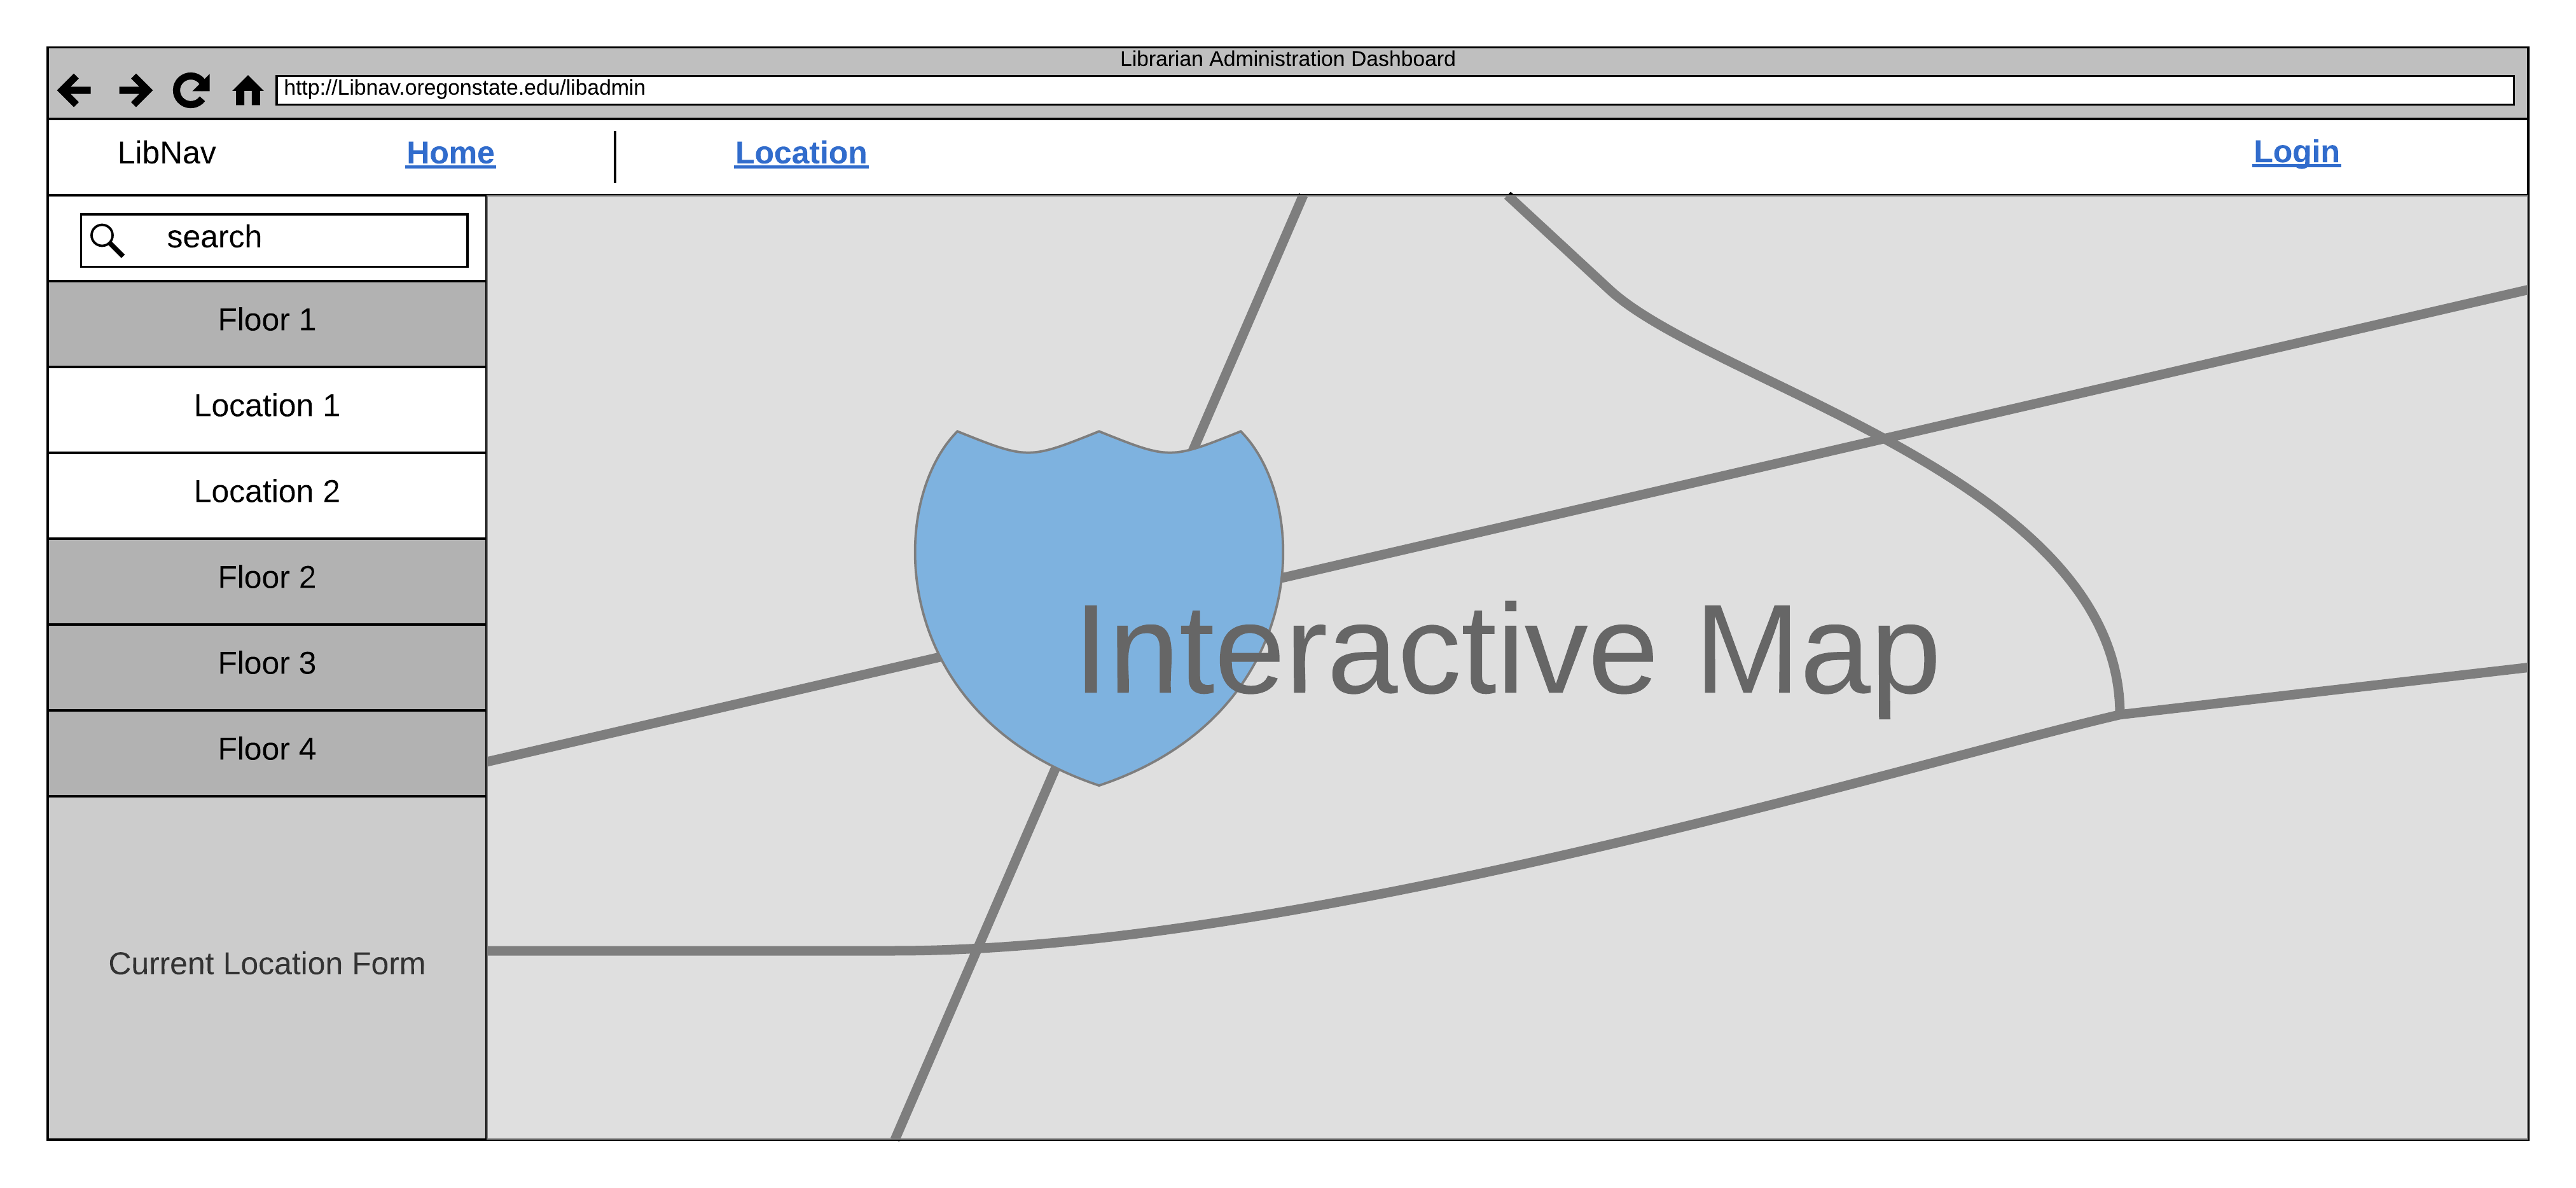
\includegraphics[scale=.45]{images/interactive-map.png}
\caption{Interactive Map User Interface}
\label{fig:method}
\end{figure}

% IM: Sidebar (Nathan)
\subsubsection{Sidebar (Nathan)}
The Sidebar the located on the left side of the Interactive Map User Interface. This design focuses on the same user as the Interface Map, technical and non-technical visitors of The Valley Library. The search consist of three areas: a search bar, Know location directory, and a Current location form. This allows user to search for location and get direction that will help them navigate to their desired destination. 

The Known location directory will allow a user to search for known location by floor then location on that floor. This will consist of a hierarchy of HTML Divs that when clicked will highlight on the map that location. When a user selects a floor and the map does not reflect that floor the map will be changed out for the correct flow. Also by clicking on a floor in the sidebar an accordion menu will open up displaying known locations of that floor. Foundation provides built in functionality for the according view but using the CSS class menu, vertical, nested.

The Current Location Form has deprecated and has been incorporated in to the functionality of the navigation. Navigation functionality allows for a user to select the point that they are current at on a grid and the desired location to be guided to.

\st{The Current Location Form allows a user to enter their current location in The Valley Library. It consists of a HTML drop down menu made of up label, select, and option tags. Valater.js will validate that a location has been selected using the isEmpty function.  A green "save" button, created using the HTML button tag, will allow a user to save the location they have selected. Once the location is saved direction will appear on the map navigation them to their desired location. A yellow "Clear" button will clear any location the user has selected along with the navigation path on the map.}

\begin{figure}[h!]
\centering
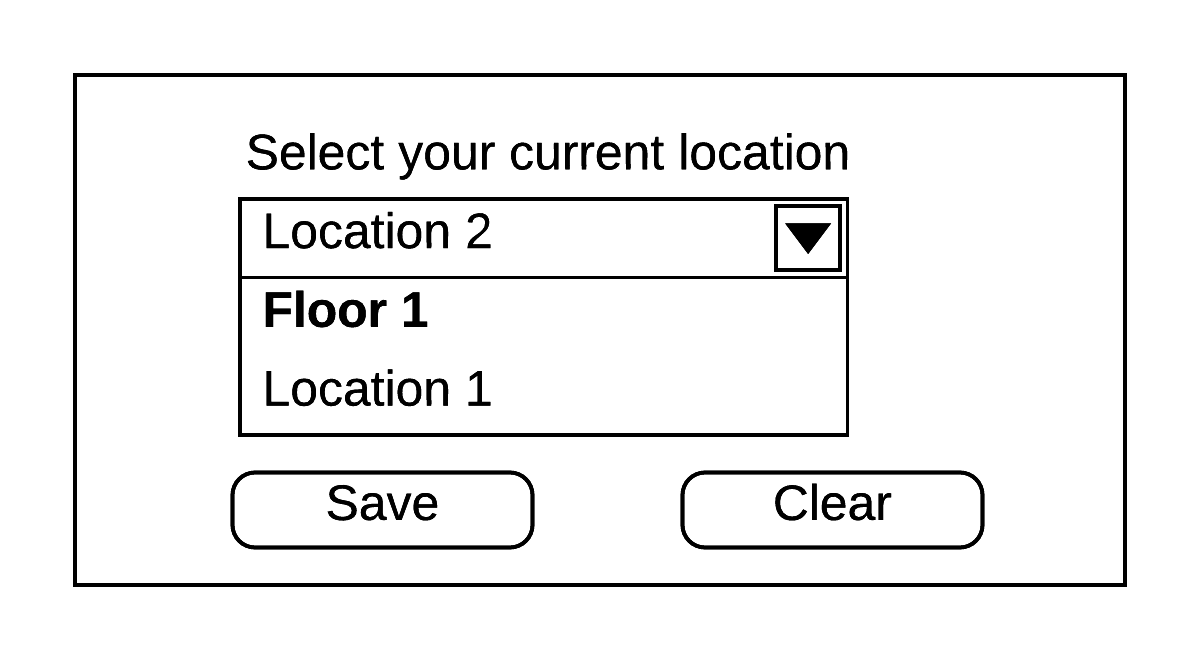
\includegraphics[]{images/current-location-form.png}
\caption{Current Location Form User Interface}
\label{fig:method}
\end{figure}

% IM: Search Bar (Matthew)
\subsubsection{Search Bar (Matthew)}
The search bar will be integrated as a part of the Interactive Map user interface. It will be found in the collapsible navigation sidebar. This will implemented as a part of the HTML and written in javascript using AngularJS plugins. The search bar will search the database tables for tags, names, and phrases associated with certain spaces. In implementation this system will use a regular expressions(RegEx) to parse through results, narrowing  down and offering options that closely match the names of spaces, any attributes or tags,  and descriptions. 

From the users' perspective, as they begin to enter a value in the search HTML search bar a drop down menu will appear with strings that contain matching substrings to the characters being entered in the search box. The RegEx search will begin to display any locations' name may match or if the substring matches any of the attributes or tags that have been assigned to a location, the names of locations with that matching tag will be displayed in the drop down list of available options. This will allow the user to search for possible locations without the need to know allow the data stored in the database or all of the locations within the library, instead only needing to know what they are looking for.

From the system perspective the search continues to query data from the database as new characters are entered into the page. Whenever a new character is entered a new query is launched to the sql database through a separate page that parses the string and receives all data returned by the query. This is parsed within the java script and then returned to the drop down menu as options for the user to select. All tags that match the string in the text box will be used to find the name of corresponding locations from the database and the location name will be given to the Javascript  to be displayed in the drop down of matching options.

% IM: Mobile View (Nathan)
\subsubsection{Mobile View (Nathan)}
The Mobile user interface is one of the main view that visitors of The Valley Library will interact. This view contains the same functionality as the Interactive Map view but scaled to fit a mobile screen. There are some modification to the side bar that will be happen but will be handled by built in functionality from Foundation. The Side navbar in the mobile view will have the option to be hidden. When this occurs a bars icon will be displayed in the upper left corner of screen. When pressed the side bar will appear and be hidden. 

\begin{figure}[h!]
\centering
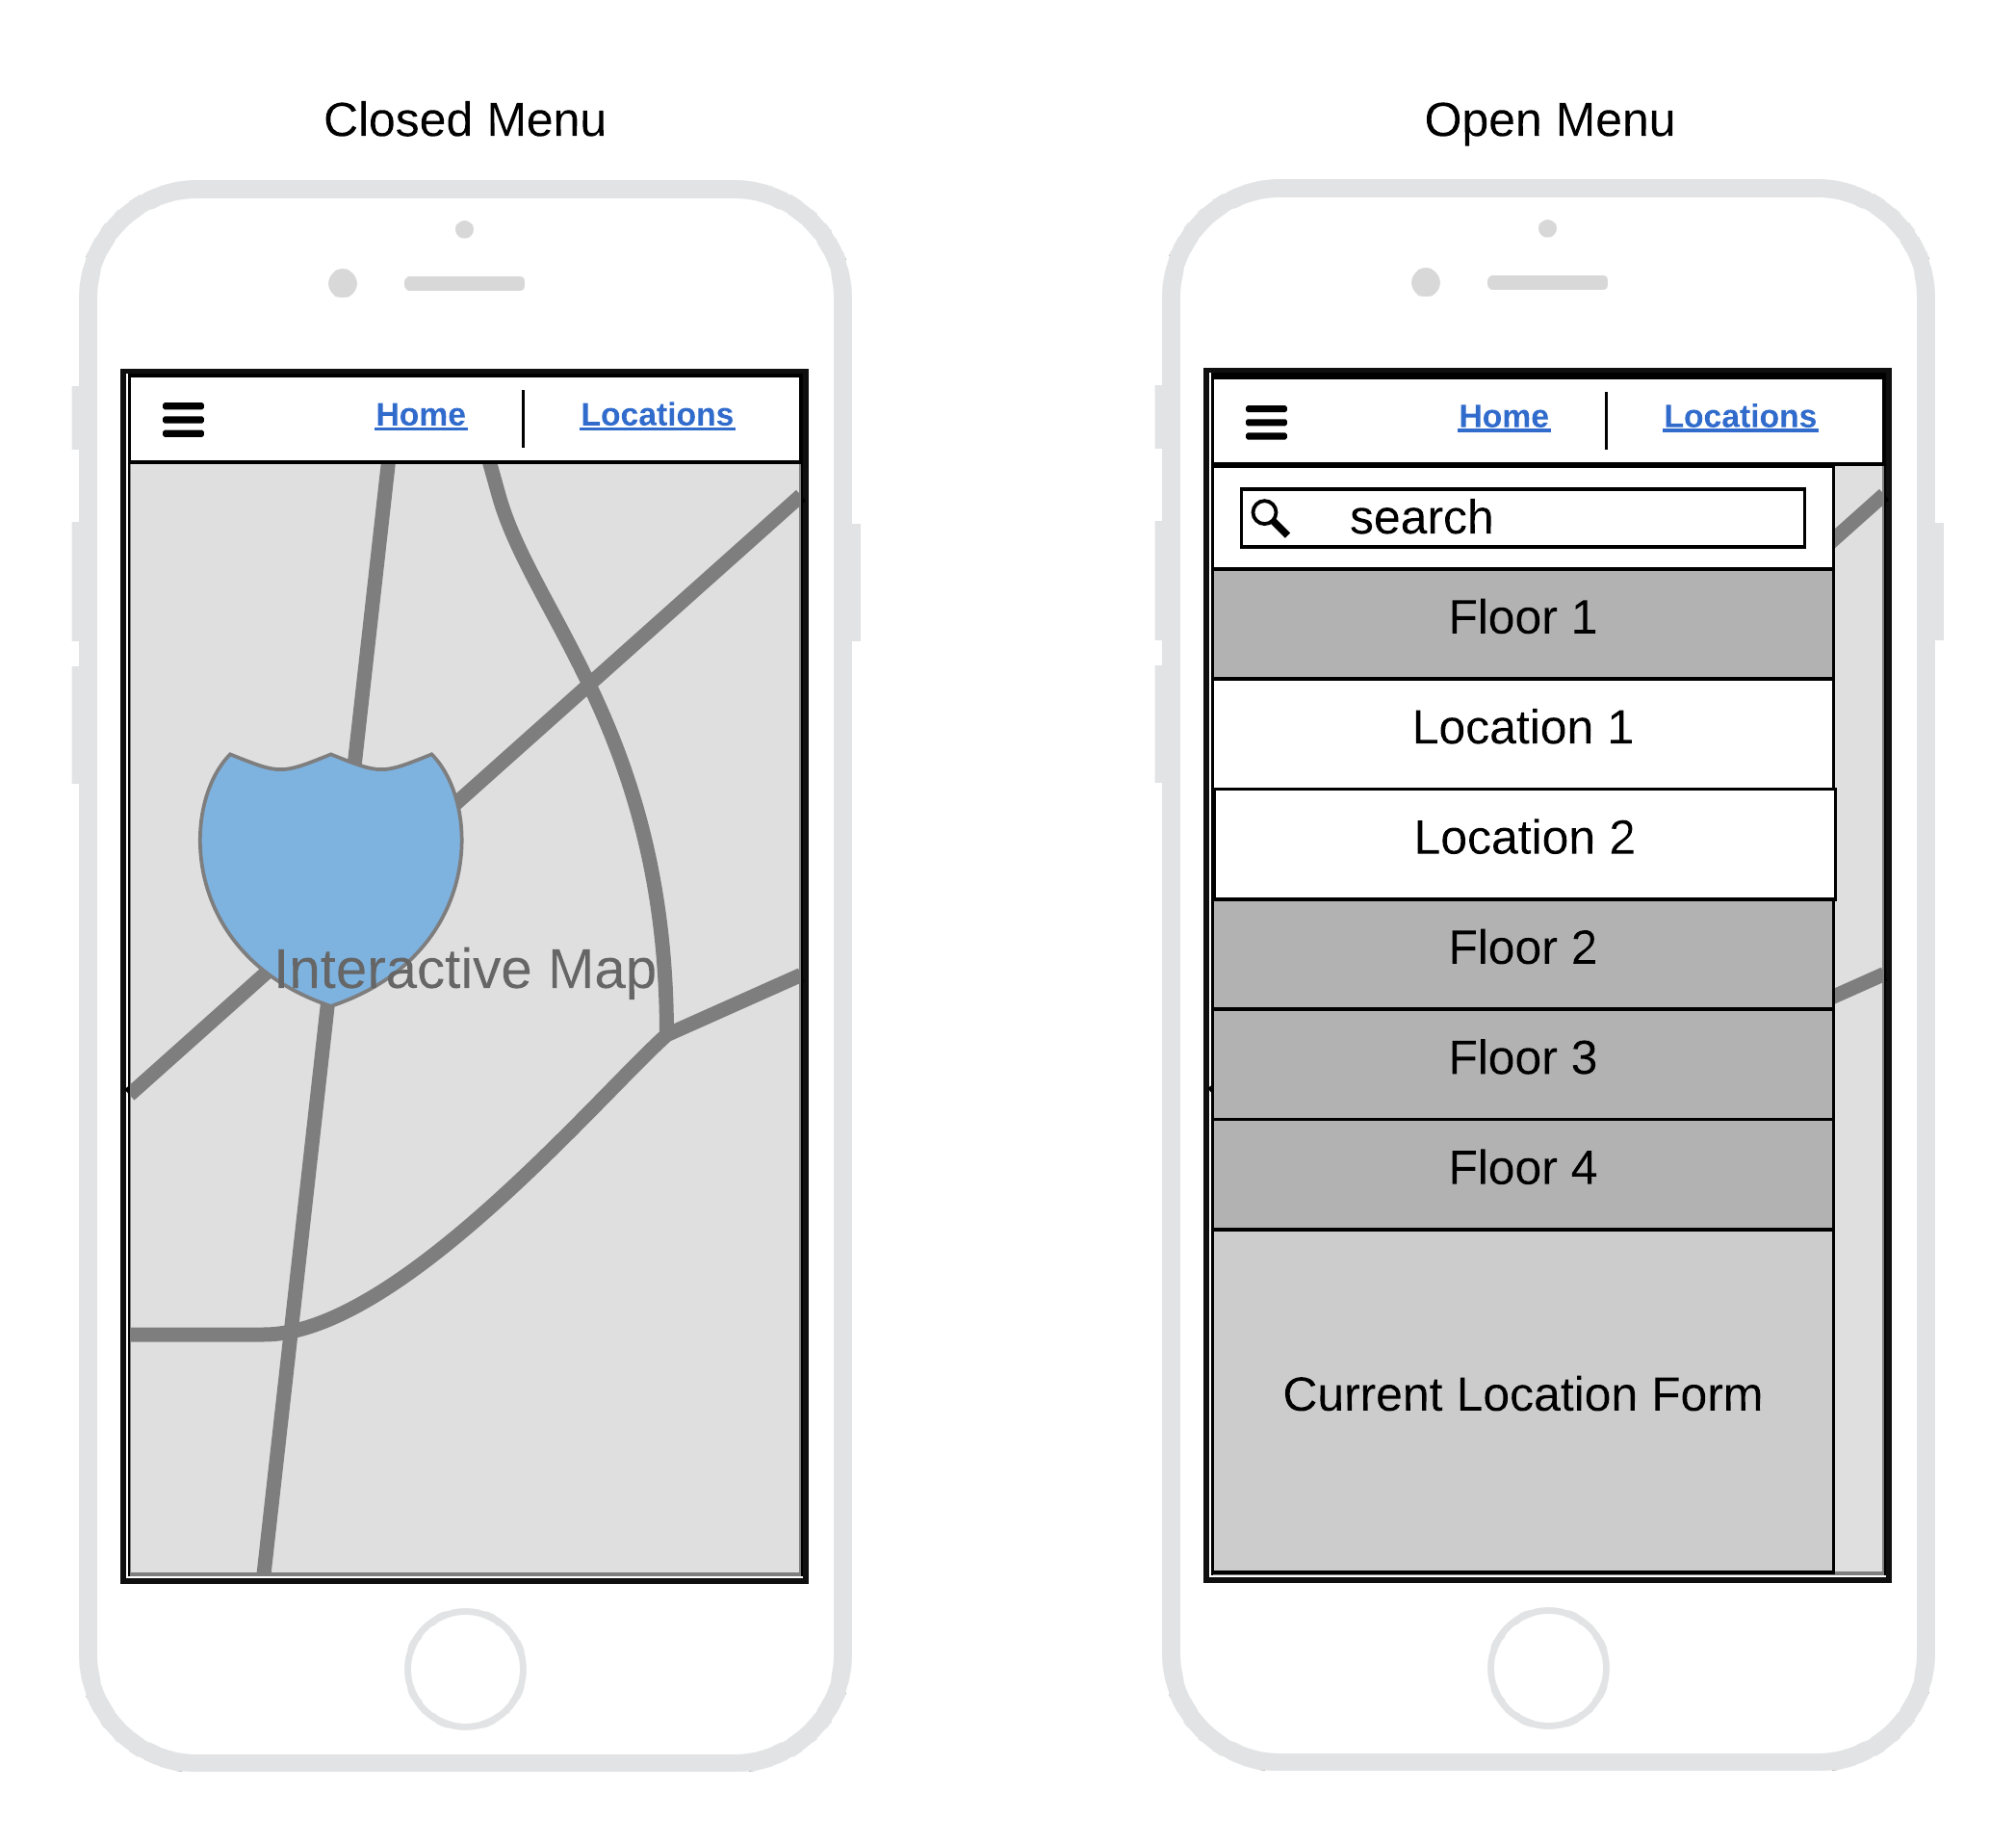
\includegraphics[scale=.6]{images/mobile-user-interface.png}
\caption{Mobile User Interface}
\label{fig:method}
\end{figure}

% IM: Map Generation (Matthew) 
\subsubsection{Map Generation (Matthew)}
For this section we will be using the D3.JS package to display our map and all of the necessary information that is saved on the map, such as the drawn shapes for each of the locations stored in the sql database. The base map image will be of the Scalable Vector Graphics(SVG) type which allow for modification and manipulation of data stored directly in the file. This map will be produced by the library staff and uploaded in the administrator dashboard. The maps will be produced on a level by level basis and will contain all of image data for each of the areas to be displayed on the map such as rooms and major landmarks. This image data will be displayed on the map with the D3.js library

The maps will each have a set size  that they will be displayed at and  through the use of onclick buttons zoom, pan, and select functions will be performed.

Basic Functions:
ZoomOutOnMap: This function take no arguments but the map will zoom out a set amount within the image space when a button is clicked. The button will look like the standard "-" buttons that are found in google maps. This will the d3.event.translate() function to perform the action.

ZoomInOnMap: This function take no arguments but the map will zoom in a set amount when a button is clicked. The button will look like the standard "+" buttons that are found in google maps. This will the d3.event.translate() function to perform the action.

Panning: will use d3.event.translate to move the map in its designated window within the web page. 

Display data(LocID):This function is used for when a person clicks on a designated space on the map and will query the database for all information that references the ID of the selected location.This will be displayed in a dynamic text box near the location selected. This data will be queried directly from the database and will be accessed through the node.js mysqljs driver.

Through the use of these functions user should have no problem navigating and viewing the map that has been created. The user should be able to freely pan and view all locations on the map. Inside the pop up text box will be a button to help populate the navigation form for route finding.

% User Login and Session (Nathan)
\section{User Login and Session (Nathan)}
The user login is designed based on existing architecture at Oregon State University.  Oregon State University uses Central Access Service (CAS) for logging in university applications. A Librarian Administrator will click a login link, displayed in the top navbar in the right corner, that will then redirect them to a CAS login screen where they will enter their ONID username and password. CAS will then verify the user login credentials and redirect the user back to the Librarian Administration Dashboard along with that user session file. If the user has access to the dashboard the user will session state will be saved if the user does not have access once the session data has been sent to the LibNav application, the user will be displayed a message indicating denial of access. This message will be shows on the homepage of the LibNav application using a Foundation modal. Yellow text will indicate that the user has been denied access. A button on the lower half of the model built using a HTML button tag  will close the modal.

Expressjs Sessions will take the user CAS session object  and store that information on the server side of the application as a session state. Then Expressjs will create a cookie in the client side that contains a hashed id. When the user interacts with the LAD the id in the session state on the server side is encrypted using the a stored key and compared to the id in the sorted cookie. If the ids match then the user will still be able to the LAD, if now the user will be redirected to home page and notified their session has expired. 

% Database (Stephen)
\section{Database (Stephen)}
The database will be an essential part of the website's functionality. Most importantly, it will store user privileges and the Grid object that the admins edit. The application will be using MySQL for all of its database needs. The database will have multiple tables that store the different information. It will pass the information back and forth as JSON objects since our backend will be using NODE.js. The map data will be stored as blobs, while user information and other extraneous information will most likely be stored as strings. Below are the different tables the application will use.
% Database: Design View (Stephen)
\subsection{Design View (Stephen)}
The Floor table will be the main table that is used to populate the maps. There will be a Location table tied to the Floor table. The location table will store the name of the room and the room number. Each location table will then a Location Attribute, Location Tags, and Gridpoint table. These three tables will store information about the location including its coordinates on the grid and the attributes the room offers. The location table also has a LocationTag table connected to it which has a Tag sub-table. These two tables will be responsible for the keyword search functionality.  These tables will not be updated or queried constantly, only when the Admin is finished and saves their work and when the floor is loaded. The other tables tied to location will be queried when the user goes to search for a room. 

Two tables, Roles and Users, will be used to store users who have admin privileges. When a new session is created, this table will be queried to determine the type of user.

\begin{figure}[h!]
\centering
\hspace*{-.5in}
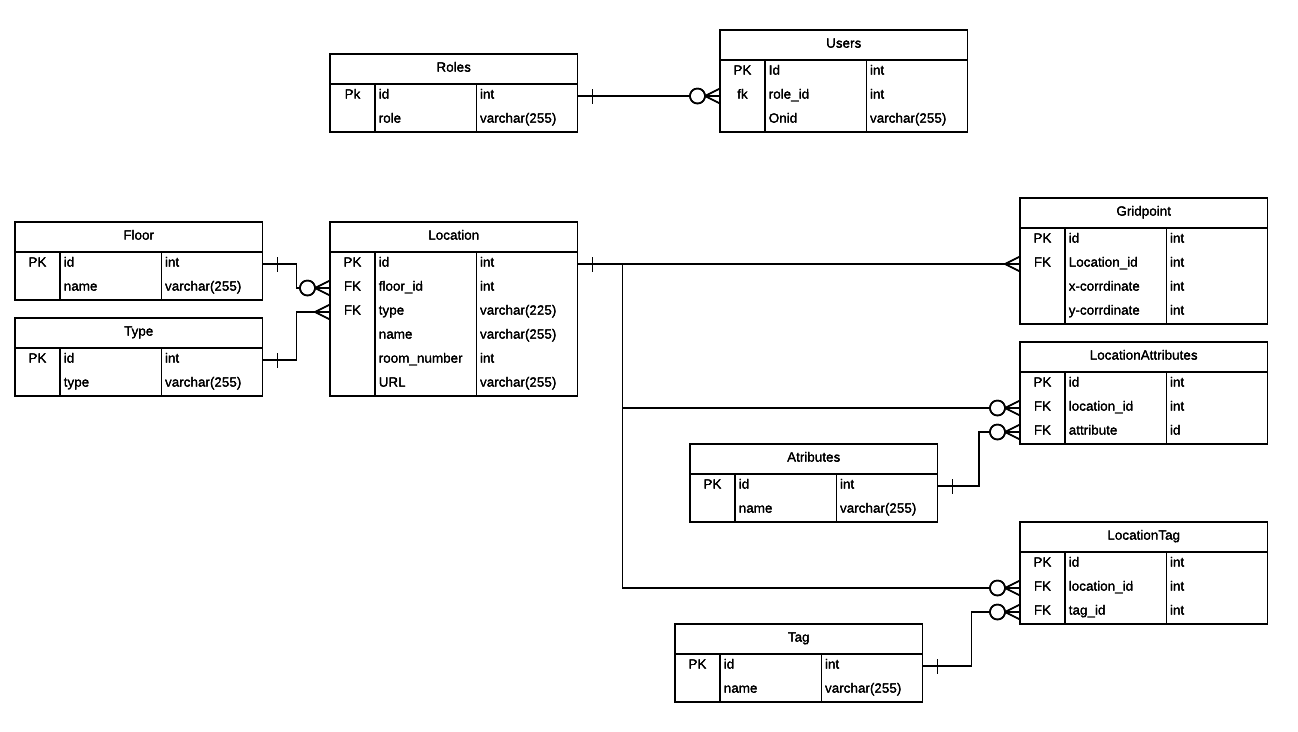
\includegraphics[scale=.65]{images/libnav-database-schema.png}
\caption{Role Assignment Form User Interface}
\label{fig:method}
\end{figure}

The node.js driver called mysqljs will be used to communicate with the database.
.connect() : The backend will connect to the database by calling the .connect() function, which takes the host, user, database password, and database name as parameters. The connection timeout can be set using the connectTimeout parameter. Connection timeout should be set to 10000 ms.




% Database: Queries
\subsection{Queries (Stephen)}
 Queries are run by calling the .query() function. Below is a list of queries that the application will be using frequently.

% Queries: Select (Stephen)
\subsubsection{Select}
\begin{enumerate}
	\item Get user info: The database will be queried to retrieve user information in JSON format. From here the application can determine user privileges.
    \item Get current map: This will return the current Grid object in JSON format.
    \item Get Keywords: Returns keywords in JSON format.
\end{enumerate}
% Queries: Update (Stephen)
\subsubsection{Update}
\begin{enumerate}
	\item Change User: This will change the current user in the session.
    \item Save Map: This will save the current map that the admin has edited.
    \item  Add Keywords: This will update the list of keywords stored in the. database
\end{enumerate}

% Queries: Delete (Stephen)
\subsubsection{Delete (Stephen)}
\begin{enumerate}
	\item Delete User: Remove user from table, stripping of admin rights.
    \item Delete Keywords: Remove keywords from the current list of keywords in the database.
\end{enumerate}


\subsection{Update (Stephen)}
Gridpoint table now stores just a json string instead of x and y coordinates. 

% Pathfinding/Navigation (PN)(Stephen)
\section{Pathfinding/Navigation (Stephen)}
The Pathfinding and Navigation feature will be responsible for finding information about desired locations on the interactive map, but also guide users from starting location to their destination. The feature will also have the ability for admins to define the paths that can be traversed throughout the library.

% NP: Design View (Stephen)
\subsection{Design View (Stephen)}
Form: The user will be presented with a form to enter in the navigation starting location and destination. The form will be built with HTML with Javascript, which will be used to implement functionality. The location and destination fields will be the only input fields on the form.  The form will capture the location and destination and send that data to the backend. The fields will implement keyword search functionality that is defined in section 3.2.2
 
Guiding Line: After the navigation path is returned by the backend functions, a blue line will appear to guide the user to their destination. The line will be traversable by the user, as in the user won’t be guided into an office or floor they can’t access.
 
Admin view: When the admin views the page they will have an ability to toggle a grid view which will present them with an overlay that shows navigable locations. On this grid they will be able to color in blocks that designate areas as un-navigable.

% NP: Backend Functions
\subsection{Backend Function (Stephen)}
Once the backend receives the data it will be sent a wayfinding function with the starting and destination locations as parameters.
 
URL inputs: The site will also take starting location inputs from URL via POST. This is so that the library can set up kiosks and QR codes with URLs that will auto-fill the starting location.
 
Function findPath((x1,y1),(x2,y2), grid) will accept two coordinate pairs and the grid. This function will plot the two points on the grid. The grid will have a list of unnavigable squares decided by the admin. The function will then use the shortest path algorithm to find the quickest path from the users starting location to their end location. It will return the traversable path and call displayPath() with a Path object as a parameter.  
 
Function displayPath(Path) will accept the Path object as a parameter. The path will be the list of coordinate pairs to be colored in. Since there should only be one path, the function will first clear any current path before coloring the grid with the new path.
 
Function clearPath() will clear the Path object.
 
Function markGrid(newPair, Grid) will accept a new coordinate pair and the Grid object as a parameter and be responsible for updating the grid every time a new coordinate pair is marked off by the admin. It returns the updated Grid object.
Function unmarkGrid(newPair, Grid) will accept a new coordinate pair and the Grid object as a parameter and be responsible for updating the grid every time a new coordinate pair is unmarked by the admin. It returns the updated Grid object.
 
Function clearGrid() will clear the Grid object.  

% Map Upload (MU)(Stephen)
\section{Map Upload (Stephen)}
The admin will need the ability to upload up to date maps to the website. The maps will be upload in a SVG image format. Each floor will need a different map and the admin needs the ability to update only one floor map at a time.  
User View:

Only the admins will be able to upload new maps. There will be a whole page of the website dedicated to uploading the maps. The library has six floors, and will therefore need at least six upload slots. Each slot will simply be an upload button and have next to it a preview of the uploaded map.

There will also be an extra slot for editing and drawing locations on new maps. The extra slot will be live but only accessible by admins. This is so that the admin can upload a new map and mark out locations, and test the map while the current floor maps are completely unchanged. Then the admin will be able to push the test slot to a floor of their choosing, overriding the old map.  

When the admin goes to upload a new map, overriding an old one, a warning message will appear asking if they’re sure that they wish to continue. The message will have two options, either update or don’t update. The admin will then be brought to a confirmation page so that they know the upload was successful.

% MU: Design View (Stephen)
\subsection{Design View (Stephen)}
The upload functionality will be handled with one main function, uploadMap().

Function uploadMap(image, floorNumber): this function will accept an image in .svg format and a floor number to designate what slot the floor will be uploaded too. It will then take the image, check if it is .svg, and save it to a folder on the server. It will then query the database and save the new image location to the correct spot in the database. Returns success call and redirects user to confirmation page. On failure it returns and displays a failure message.

Function deleteMap(floorNumber): this function will delete the map that is saved for the floor number that is accepted as a parameter. It will clear the image in the server as well as the location tied to the database. Returns success message and redirects user to confirmation page. On failure it returns and displays a failure message.

Function pushLive(floorNumber): this function accepts a floor number as a parameter. This is the function that will push the test slot live. It will then take the map in the test slot and push it to the slot of whatever floor number is specified. Returns success message and redirects user to confirmation page. On failure it returns and displays a failure message.

\newpage
% Bibliography
%\section{Bibliography}
%\bibliographystyle{IEEEtran}
%\bibliography{bibiography.bib}

% Section: Signatures
\section*{Signatures}

\subsection*{Client}
\vspace{10mm} %5mm vertical space
\noindent\begin{tabular}{ll}
\makebox[2.5in]{\hrulefill} & \makebox[2.5in]{\hrulefill}\\
Beth Filar Williams & Date\\[8ex]
\end{tabular}

\subsection*{Capstone Team}
\vspace{10mm} %5mm vertical space
\noindent\begin{tabular}{ll}
\makebox[2.5in]{\hrulefill} & \makebox[2.5in]{\hrulefill}\\
Nathan Healea & Date\\[8ex]
\makebox[2.5in]{\hrulefill} & \makebox[2.5in]{\hrulefill}\\
Stephen Krueger & Date\\[8ex]
\makebox[2.5in]{\hrulefill} & \makebox[2.5in]{\hrulefill}\\
Matthew Zakrevsky & Date\\[8ex]

\end{tabular}


\end{document}
